\documentclass[a4paper,10pt]{article}
%\documentclass[a4paper,10pt]{scrartcl}

\usepackage[utf8x]{inputenc}
\usepackage{amsmath}
 \usepackage{graphicx}

\title{HW\#3-P1}
\author{Christopher Stricklan}
\date{02/13/2011}

\pdfinfo{%
  /Title    (HW#3-P1)
  /Author   (Christopher Stricklan)
  /Creator  (Christopher Stricklan)
  /Producer (Christopher Stricklan)
  /Subject  (EE5390-FDTD)
  /Keywords (FDTD)
}

\begin{document}
%\maketitle
\textbf{Maxwell's Equations}

\begin{equation}
  \nabla \cdot \vec{D}(t)=\rho_{v}(t)
\end{equation}

\begin{equation}
  \nabla \cdot \vec{B}(t)=0
\end{equation}

\begin{equation}
  \nabla \times \vec{E}(t) = -\frac{\partial \vec{B}(t)}{\partial t}
\end{equation}

\begin{equation}
  \nabla \times \vec{H}(t) = \vec{J} + \frac{\partial\vec{D}(t)}{\partial t}
\end{equation}
                                                                                   

\textbf{Constitutive relations}
\begin{equation}
  \label{eq:constitutive1}
  \vec{D} = [\epsilon(t)]*\vec{E}(t)
\end{equation}

\begin{equation}
  \label{eq:constitutive2}
  \vec{B} = [\mu(t)]*\vec{H}(t)
\end{equation}


\textbf{Eliminate Divergence}

Our use of the Yee Grid Scheme alows us to elimate divergence via equations \eqref{eq:Divergence1} and \eqref{eq:Divergence2}

\begin{equation} 
  \label{eq:Divergence1}
  \nabla \cdot (\epsilon\vec{E}) = 0
\end{equation}

\begin{equation} 
  \label{eq:Divergence2}
  \nabla \cdot(\mu\vec{H}) = 0
\end{equation}

This also allows for the centering of the fields invoked by the curl equations Figure \ref{fig:YeeGridWithCurls}

\begin{figure}[h]
  \centering
    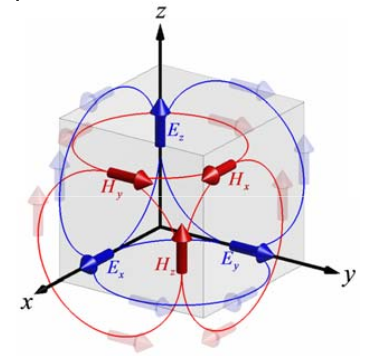
\includegraphics[width=0.5\textwidth]{YeeGrid.png}
  \caption{Yee Grid}
  \label{fig:YeeGridWithCurls}
\end{figure}
	

\textbf{Substitution}

Because we have satisfied the divergence equations by using the Yee Grid Scheme, we are now able to focus on the curl equations with our constituive relation equations \eqref{eq:constitutive1} and \eqref{eq:constitutive2} subsituted in.  We are also not injecting a Source.

\begin{equation*}
 \mbox{Where }\vec{J} = 0
\end{equation*}


\begin{equation}
  \nabla \times \vec{E}(t) = -[\mu]\frac{\partial \vec{H}(t)}{\partial t}
\end{equation}


\begin{equation}
   \nabla \times \vec{H}(t) = [\epsilon]\frac{\partial\vec{H}(t)}{\partial t}
\end{equation}


\textbf{Normalize Magnetic Field}

The Electric and Magnetic Fields are three orders of magnitude different.  Rounding errors can propagate through our simulation, therefore we require that we normalize a Field.  In this case we are normalizing the Magnetic Field.

\begin{equation}
  \vec{\tilde{H}} = \sqrt{\frac{\mu_0}{\epsilon_0}}\vec{H}
\end{equation}























































\end{document}

